% Requires:
% \usepackage{pgfplots}
% \usepackage{siunitx}
% \pgfplotsset{compat=1.18}
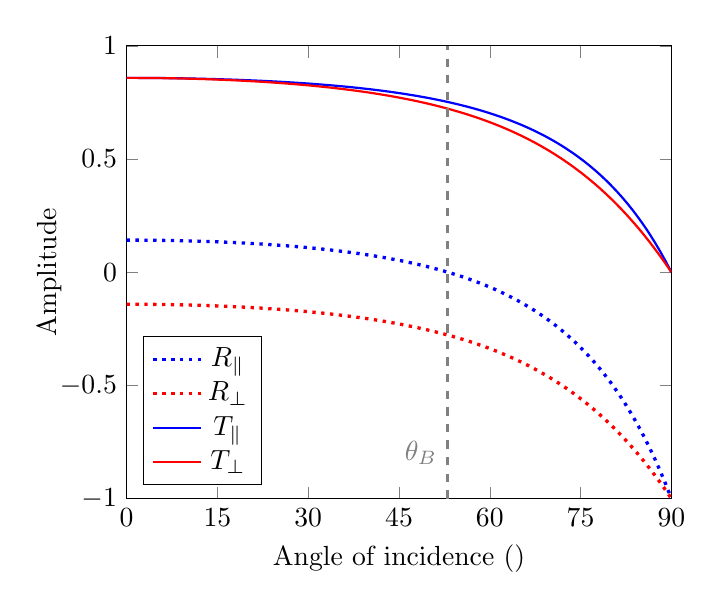
\begin{tikzpicture}
  \begin{axis}[
      xlabel={Angle of incidence (\unit{\degree})},
      ylabel={Amplitude},
      %ylabel style={yshift=-1em},
      every axis y label/.append style={at={([xshift=-2em]ticklabel* cs:.5)}},
      width=8.5cm,
      xmin=0, xmax=90,
      xtick={0, 15, 30, 45, 60, 75, 90},
      ymin=-1.0, ymax=1.0,
      legend pos=south west,
      /pgf/declare function={
        n = 1.33; % Refractive index ratio n_water / n_air
        % Intermediate term: n_r * cos(theta_t) = sqrt(n^2 - sin(x)^2)
        n_cos_t(\x) = sqrt(n^2 - (sin(\x))^2);
        % Fresnel equations
        rs(\x) = (cos(\x) - n_cos_t(\x)) / (cos(\x) + n_cos_t(\x));
        rp(\x) = (n^2 * cos(\x) - n_cos_t(\x)) / (n^2 * cos(\x) + n_cos_t(\x));
        ts(\x) = (2 * cos(\x)) / (cos(\x) + n_cos_t(\x));
        tp(\x) = (2 * n * cos(\x)) / (n^2 * cos(\x) + n_cos_t(\x));
        % Brewster angle
        thetaB = atan(n);
      }
    ]
    \addplot[blue, dotted, very thick, domain=0:90, samples=100] {rp(x)};
    \addlegendentry{$R_\parallel$}

    \addplot[red, dotted, very thick, domain=0:90, samples=100] {rs(x)};
    \addlegendentry{$R_\perp$}

    \addplot[blue, solid, thick, domain=0:90, samples=100] {tp(x)};
    \addlegendentry{$T_\parallel$}

    \addplot[red, solid, thick, domain=0:90, samples=100] {ts(x)};
    \addlegendentry{$T_\perp$}

    % Vertical line for Brewster angle
    \addplot [gray, very thick, dashed, update limits=false] coordinates {(thetaB, -1) (thetaB, 1)} node[pos=.1, left] {$\theta_B$};
  \end{axis}
\end{tikzpicture}
